% !TEX encoding = UTF-8 Unicode
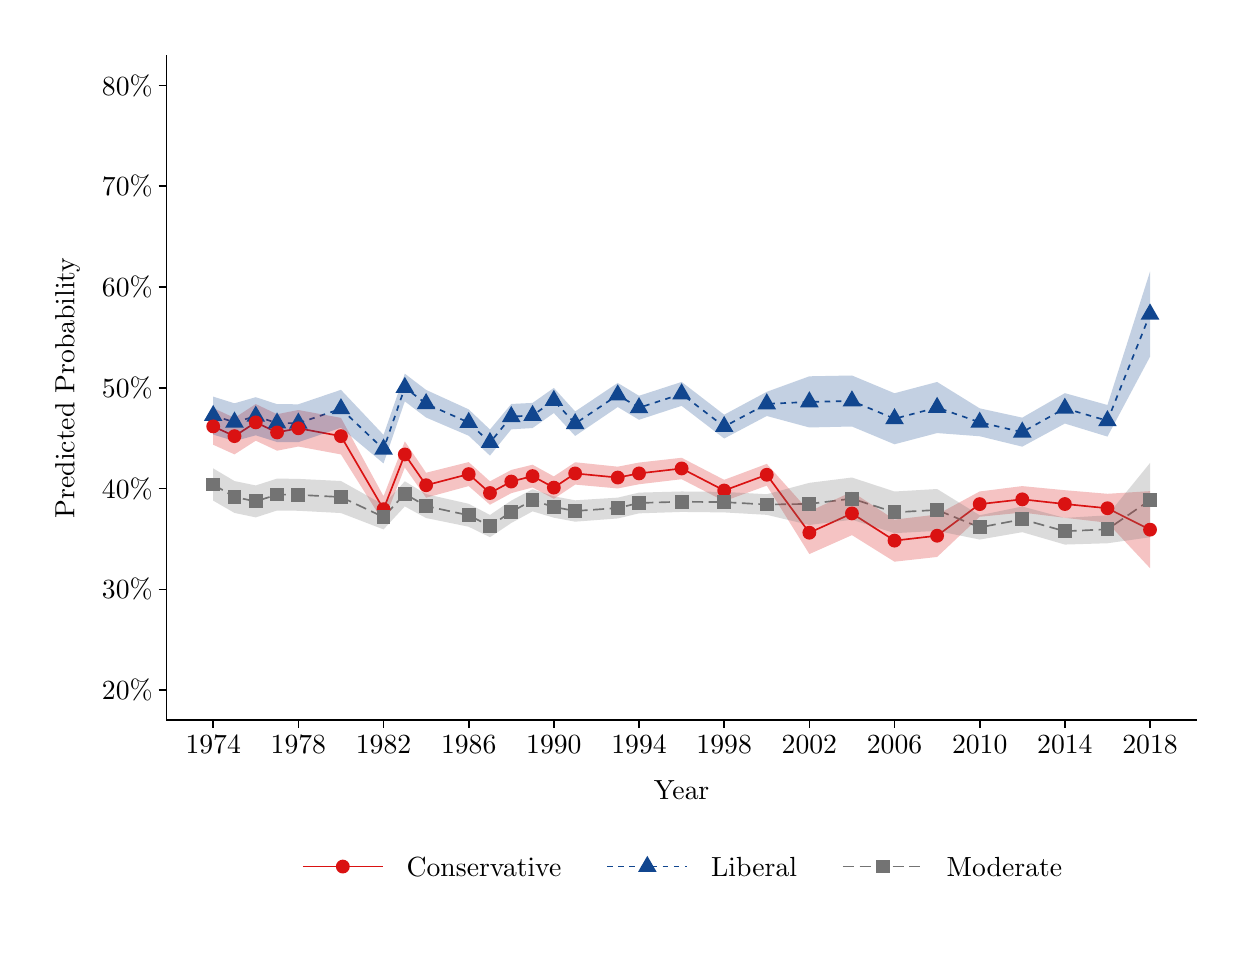
\begin{tikzpicture}[x=1pt,y=1pt]
\definecolor{fillColor}{RGB}{255,255,255}
\path[use as bounding box,fill=fillColor,fill opacity=0.00] (0,0) rectangle (432.48,324.36);
\begin{scope}
\path[clip] (  0.00,  0.00) rectangle (432.48,324.36);
\definecolor{fillColor}{RGB}{255,255,255}

\path[fill=fillColor] ( -0.00,  0.00) rectangle (432.48,324.36);
\end{scope}
\begin{scope}
\path[clip] ( 50.11, 74.07) rectangle (422.48,314.36);
\definecolor{fillColor}{RGB}{255,255,255}

\path[fill=fillColor] ( 50.11, 74.07) rectangle (422.48,314.36);
\definecolor{drawColor}{RGB}{218,18,18}

\path[draw=drawColor,line width= 0.6pt,line join=round] ( 67.04,180.28) --
	( 74.73,176.76) --
	( 82.42,181.73) --
	( 90.12,178.10) --
	( 97.81,179.60) --
	(113.20,176.76) --
	(128.59,150.37) --
	(136.28,170.14) --
	(143.97,159.02) --
	(159.36,163.04) --
	(167.05,156.20) --
	(174.75,160.35) --
	(182.44,162.32) --
	(190.13,158.16) --
	(197.83,163.28) --
	(213.22,161.79) --
	(220.91,163.29) --
	(236.30,165.07) --
	(251.68,157.11) --
	(267.07,162.80) --
	(282.46,141.86) --
	(297.85,148.83) --
	(313.23,139.00) --
	(328.62,140.77) --
	(344.01,152.20) --
	(359.39,153.92) --
	(374.78,152.23) --
	(390.17,150.70) --
	(405.56,142.96);
\definecolor{drawColor}{RGB}{17,70,143}

\path[draw=drawColor,line width= 0.6pt,dash pattern=on 2pt off 2pt ,line join=round] ( 67.04,184.17) --
	( 74.73,181.80) --
	( 82.42,183.94) --
	( 90.12,181.47) --
	( 97.81,181.43) --
	(113.20,186.64) --
	(128.59,172.04) --
	(136.28,194.32) --
	(143.97,188.47) --
	(159.36,181.67) --
	(167.05,174.43) --
	(174.75,183.80) --
	(182.44,184.22) --
	(190.13,189.64) --
	(197.83,181.26) --
	(213.22,191.62) --
	(220.91,187.01) --
	(236.30,192.02) --
	(251.68,180.20) --
	(267.07,188.41) --
	(282.46,189.13) --
	(297.85,189.46) --
	(313.23,183.04) --
	(328.62,187.10) --
	(344.01,181.76) --
	(359.39,178.20) --
	(374.78,186.80) --
	(390.17,182.31) --
	(405.56,220.84);
\definecolor{drawColor}{gray}{0.45}

\path[draw=drawColor,line width= 0.6pt,dash pattern=on 4pt off 2pt ,line join=round] ( 67.04,159.28) --
	( 74.73,154.77) --
	( 82.42,153.17) --
	( 90.12,155.65) --
	( 97.81,155.55) --
	(113.20,154.75) --
	(128.59,147.52) --
	(136.28,155.91) --
	(143.97,151.48) --
	(159.36,148.16) --
	(167.05,144.26) --
	(174.75,149.43) --
	(182.44,153.57) --
	(190.13,151.16) --
	(197.83,149.71) --
	(213.22,150.78) --
	(220.91,152.61) --
	(236.30,153.06) --
	(251.68,152.91) --
	(267.07,152.04) --
	(282.46,152.27) --
	(297.85,154.18) --
	(313.23,149.23) --
	(328.62,150.09) --
	(344.01,143.78) --
	(359.39,146.70) --
	(374.78,142.39) --
	(390.17,143.10) --
	(405.56,153.64);
\definecolor{fillColor}{RGB}{218,18,18}

\path[fill=fillColor,fill opacity=0.25] ( 67.04,186.91) --
	( 74.73,183.36) --
	( 82.42,188.35) --
	( 90.12,184.69) --
	( 97.81,186.20) --
	(113.20,183.37) --
	(128.59,155.04) --
	(136.28,174.86) --
	(143.97,163.52) --
	(159.36,167.37) --
	(167.05,160.43) --
	(174.75,164.54) --
	(182.44,166.43) --
	(190.13,162.20) --
	(197.83,167.32) --
	(213.22,165.72) --
	(220.91,167.21) --
	(236.30,168.94) --
	(251.68,160.97) --
	(267.07,166.73) --
	(282.46,149.56) --
	(297.85,156.67) --
	(313.23,146.60) --
	(328.62,148.43) --
	(344.01,156.77) --
	(359.39,158.70) --
	(374.78,157.22) --
	(390.17,155.92) --
	(405.56,156.88) --
	(405.56,129.05) --
	(390.17,145.48) --
	(374.78,147.25) --
	(359.39,149.15) --
	(344.01,147.62) --
	(328.62,133.10) --
	(313.23,131.39) --
	(297.85,140.99) --
	(282.46,134.15) --
	(267.07,158.87) --
	(251.68,153.26) --
	(236.30,161.20) --
	(220.91,159.37) --
	(213.22,157.86) --
	(197.83,159.25) --
	(190.13,154.12) --
	(182.44,158.22) --
	(174.75,156.16) --
	(167.05,151.98) --
	(159.36,158.71) --
	(143.97,154.52) --
	(136.28,165.43) --
	(128.59,145.69) --
	(113.20,170.15) --
	( 97.81,173.01) --
	( 90.12,171.50) --
	( 82.42,175.11) --
	( 74.73,170.17) --
	( 67.04,173.65) --
	cycle;

\path[] ( 67.04,186.91) --
	( 74.73,183.36) --
	( 82.42,188.35) --
	( 90.12,184.69) --
	( 97.81,186.20) --
	(113.20,183.37) --
	(128.59,155.04) --
	(136.28,174.86) --
	(143.97,163.52) --
	(159.36,167.37) --
	(167.05,160.43) --
	(174.75,164.54) --
	(182.44,166.43) --
	(190.13,162.20) --
	(197.83,167.32) --
	(213.22,165.72) --
	(220.91,167.21) --
	(236.30,168.94) --
	(251.68,160.97) --
	(267.07,166.73) --
	(282.46,149.56) --
	(297.85,156.67) --
	(313.23,146.60) --
	(328.62,148.43) --
	(344.01,156.77) --
	(359.39,158.70) --
	(374.78,157.22) --
	(390.17,155.92) --
	(405.56,156.88);

\path[] (405.56,129.05) --
	(390.17,145.48) --
	(374.78,147.25) --
	(359.39,149.15) --
	(344.01,147.62) --
	(328.62,133.10) --
	(313.23,131.39) --
	(297.85,140.99) --
	(282.46,134.15) --
	(267.07,158.87) --
	(251.68,153.26) --
	(236.30,161.20) --
	(220.91,159.37) --
	(213.22,157.86) --
	(197.83,159.25) --
	(190.13,154.12) --
	(182.44,158.22) --
	(174.75,156.16) --
	(167.05,151.98) --
	(159.36,158.71) --
	(143.97,154.52) --
	(136.28,165.43) --
	(128.59,145.69) --
	(113.20,170.15) --
	( 97.81,173.01) --
	( 90.12,171.50) --
	( 82.42,175.11) --
	( 74.73,170.17) --
	( 67.04,173.65);
\definecolor{fillColor}{RGB}{17,70,143}

\path[fill=fillColor,fill opacity=0.25] ( 67.04,191.03) --
	( 74.73,188.62) --
	( 82.42,190.83) --
	( 90.12,188.31) --
	( 97.81,188.27) --
	(113.20,193.49) --
	(128.59,177.20) --
	(136.28,199.32) --
	(143.97,193.46) --
	(159.36,186.44) --
	(167.05,179.14) --
	(174.75,188.38) --
	(182.44,188.77) --
	(190.13,194.17) --
	(197.83,185.69) --
	(213.22,195.97) --
	(220.91,191.34) --
	(236.30,196.34) --
	(251.68,184.50) --
	(267.07,192.78) --
	(282.46,198.38) --
	(297.85,198.67) --
	(313.23,192.26) --
	(328.62,196.33) --
	(344.01,186.80) --
	(359.39,183.44) --
	(374.78,192.29) --
	(390.17,188.01) --
	(405.56,236.23) --
	(405.56,205.46) --
	(390.17,176.60) --
	(374.78,181.31) --
	(359.39,172.96) --
	(344.01,176.72) --
	(328.62,177.87) --
	(313.23,173.82) --
	(297.85,180.24) --
	(282.46,179.89) --
	(267.07,184.04) --
	(251.68,175.90) --
	(236.30,187.71) --
	(220.91,182.67) --
	(213.22,187.27) --
	(197.83,176.83) --
	(190.13,185.11) --
	(182.44,179.68) --
	(174.75,179.22) --
	(167.05,169.72) --
	(159.36,176.90) --
	(143.97,183.48) --
	(136.28,189.32) --
	(128.59,166.89) --
	(113.20,179.79) --
	( 97.81,174.59) --
	( 90.12,174.63) --
	( 82.42,177.05) --
	( 74.73,174.98) --
	( 67.04,177.31) --
	cycle;

\path[] ( 67.04,191.03) --
	( 74.73,188.62) --
	( 82.42,190.83) --
	( 90.12,188.31) --
	( 97.81,188.27) --
	(113.20,193.49) --
	(128.59,177.20) --
	(136.28,199.32) --
	(143.97,193.46) --
	(159.36,186.44) --
	(167.05,179.14) --
	(174.75,188.38) --
	(182.44,188.77) --
	(190.13,194.17) --
	(197.83,185.69) --
	(213.22,195.97) --
	(220.91,191.34) --
	(236.30,196.34) --
	(251.68,184.50) --
	(267.07,192.78) --
	(282.46,198.38) --
	(297.85,198.67) --
	(313.23,192.26) --
	(328.62,196.33) --
	(344.01,186.80) --
	(359.39,183.44) --
	(374.78,192.29) --
	(390.17,188.01) --
	(405.56,236.23);

\path[] (405.56,205.46) --
	(390.17,176.60) --
	(374.78,181.31) --
	(359.39,172.96) --
	(344.01,176.72) --
	(328.62,177.87) --
	(313.23,173.82) --
	(297.85,180.24) --
	(282.46,179.89) --
	(267.07,184.04) --
	(251.68,175.90) --
	(236.30,187.71) --
	(220.91,182.67) --
	(213.22,187.27) --
	(197.83,176.83) --
	(190.13,185.11) --
	(182.44,179.68) --
	(174.75,179.22) --
	(167.05,169.72) --
	(159.36,176.90) --
	(143.97,183.48) --
	(136.28,189.32) --
	(128.59,166.89) --
	(113.20,179.79) --
	( 97.81,174.59) --
	( 90.12,174.63) --
	( 82.42,177.05) --
	( 74.73,174.98) --
	( 67.04,177.31);
\definecolor{fillColor}{RGB}{115,115,115}

\path[fill=fillColor,fill opacity=0.25] ( 67.04,165.10) --
	( 74.73,160.53) --
	( 82.42,158.94) --
	( 90.12,161.42) --
	( 97.81,161.31) --
	(113.20,160.54) --
	(128.59,151.98) --
	(136.28,160.45) --
	(143.97,155.80) --
	(159.36,152.31) --
	(167.05,148.28) --
	(174.75,153.48) --
	(182.44,157.56) --
	(190.13,155.02) --
	(197.83,153.57) --
	(213.22,154.54) --
	(220.91,156.35) --
	(236.30,156.76) --
	(251.68,156.62) --
	(267.07,155.76) --
	(282.46,159.88) --
	(297.85,161.80) --
	(313.23,156.75) --
	(328.62,157.65) --
	(344.01,148.17) --
	(359.39,151.33) --
	(374.78,147.20) --
	(390.17,148.15) --
	(405.56,167.06) --
	(405.56,140.22) --
	(390.17,138.05) --
	(374.78,137.58) --
	(359.39,142.06) --
	(344.01,139.39) --
	(328.62,142.53) --
	(313.23,141.70) --
	(297.85,146.56) --
	(282.46,144.66) --
	(267.07,148.32) --
	(251.68,149.20) --
	(236.30,149.37) --
	(220.91,148.86) --
	(213.22,147.02) --
	(197.83,145.85) --
	(190.13,147.29) --
	(182.44,149.58) --
	(174.75,145.38) --
	(167.05,140.24) --
	(159.36,144.02) --
	(143.97,147.17) --
	(136.28,151.37) --
	(128.59,143.06) --
	(113.20,148.97) --
	( 97.81,149.79) --
	( 90.12,149.89) --
	( 82.42,147.40) --
	( 74.73,149.01) --
	( 67.04,153.46) --
	cycle;

\path[] ( 67.04,165.10) --
	( 74.73,160.53) --
	( 82.42,158.94) --
	( 90.12,161.42) --
	( 97.81,161.31) --
	(113.20,160.54) --
	(128.59,151.98) --
	(136.28,160.45) --
	(143.97,155.80) --
	(159.36,152.31) --
	(167.05,148.28) --
	(174.75,153.48) --
	(182.44,157.56) --
	(190.13,155.02) --
	(197.83,153.57) --
	(213.22,154.54) --
	(220.91,156.35) --
	(236.30,156.76) --
	(251.68,156.62) --
	(267.07,155.76) --
	(282.46,159.88) --
	(297.85,161.80) --
	(313.23,156.75) --
	(328.62,157.65) --
	(344.01,148.17) --
	(359.39,151.33) --
	(374.78,147.20) --
	(390.17,148.15) --
	(405.56,167.06);

\path[] (405.56,140.22) --
	(390.17,138.05) --
	(374.78,137.58) --
	(359.39,142.06) --
	(344.01,139.39) --
	(328.62,142.53) --
	(313.23,141.70) --
	(297.85,146.56) --
	(282.46,144.66) --
	(267.07,148.32) --
	(251.68,149.20) --
	(236.30,149.37) --
	(220.91,148.86) --
	(213.22,147.02) --
	(197.83,145.85) --
	(190.13,147.29) --
	(182.44,149.58) --
	(174.75,145.38) --
	(167.05,140.24) --
	(159.36,144.02) --
	(143.97,147.17) --
	(136.28,151.37) --
	(128.59,143.06) --
	(113.20,148.97) --
	( 97.81,149.79) --
	( 90.12,149.89) --
	( 82.42,147.40) --
	( 74.73,149.01) --
	( 67.04,153.46);
\definecolor{fillColor}{RGB}{17,70,143}

\path[fill=fillColor] ( 67.04,188.05) --
	( 70.40,182.23) --
	( 63.67,182.23) --
	cycle;

\path[fill=fillColor] ( 74.73,185.69) --
	( 78.09,179.86) --
	( 71.37,179.86) --
	cycle;

\path[fill=fillColor] ( 82.42,187.82) --
	( 85.79,182.00) --
	( 79.06,182.00) --
	cycle;

\path[fill=fillColor] ( 90.12,185.35) --
	( 93.48,179.53) --
	( 86.75,179.53) --
	cycle;

\path[fill=fillColor] ( 97.81,185.32) --
	(101.17,179.49) --
	( 94.45,179.49) --
	cycle;

\path[fill=fillColor] (113.20,190.52) --
	(116.56,184.70) --
	(109.83,184.70) --
	cycle;

\path[fill=fillColor] (128.59,175.93) --
	(131.95,170.10) --
	(125.22,170.10) --
	cycle;

\path[fill=fillColor] (136.28,198.20) --
	(139.64,192.38) --
	(132.91,192.38) --
	cycle;

\path[fill=fillColor] (143.97,192.35) --
	(147.34,186.53) --
	(140.61,186.53) --
	cycle;

\path[fill=fillColor] (159.36,185.56) --
	(162.72,179.73) --
	(156.00,179.73) --
	cycle;

\path[fill=fillColor] (167.05,178.31) --
	(170.42,172.49) --
	(163.69,172.49) --
	cycle;

\path[fill=fillColor] (174.75,187.68) --
	(178.11,181.86) --
	(171.38,181.86) --
	cycle;

\path[fill=fillColor] (182.44,188.11) --
	(185.80,182.28) --
	(179.08,182.28) --
	cycle;

\path[fill=fillColor] (190.13,193.52) --
	(193.50,187.70) --
	(186.77,187.70) --
	cycle;

\path[fill=fillColor] (197.83,185.14) --
	(201.19,179.32) --
	(194.46,179.32) --
	cycle;

\path[fill=fillColor] (213.22,195.50) --
	(216.58,189.68) --
	(209.85,189.68) --
	cycle;

\path[fill=fillColor] (220.91,190.89) --
	(224.27,185.06) --
	(217.54,185.06) --
	cycle;

\path[fill=fillColor] (236.30,195.91) --
	(239.66,190.08) --
	(232.93,190.08) --
	cycle;

\path[fill=fillColor] (251.68,184.09) --
	(255.05,178.26) --
	(248.32,178.26) --
	cycle;

\path[fill=fillColor] (267.07,192.30) --
	(270.43,186.47) --
	(263.71,186.47) --
	cycle;

\path[fill=fillColor] (282.46,193.02) --
	(285.82,187.19) --
	(279.09,187.19) --
	cycle;

\path[fill=fillColor] (297.85,193.34) --
	(301.21,187.51) --
	(294.48,187.51) --
	cycle;

\path[fill=fillColor] (313.23,186.92) --
	(316.60,181.10) --
	(309.87,181.10) --
	cycle;

\path[fill=fillColor] (328.62,190.99) --
	(331.98,185.16) --
	(325.26,185.16) --
	cycle;

\path[fill=fillColor] (344.01,185.64) --
	(347.37,179.82) --
	(340.64,179.82) --
	cycle;

\path[fill=fillColor] (359.39,182.08) --
	(362.76,176.26) --
	(356.03,176.26) --
	cycle;

\path[fill=fillColor] (374.78,190.68) --
	(378.15,184.86) --
	(371.42,184.86) --
	cycle;

\path[fill=fillColor] (390.17,186.19) --
	(393.53,180.36) --
	(386.80,180.36) --
	cycle;

\path[fill=fillColor] (405.56,224.73) --
	(408.92,218.90) --
	(402.19,218.90) --
	cycle;
\definecolor{fillColor}{RGB}{218,18,18}

\path[fill=fillColor] ( 67.04,180.28) circle (  2.50);

\path[fill=fillColor] ( 74.73,176.76) circle (  2.50);

\path[fill=fillColor] ( 82.42,181.73) circle (  2.50);

\path[fill=fillColor] ( 90.12,178.10) circle (  2.50);

\path[fill=fillColor] ( 97.81,179.60) circle (  2.50);

\path[fill=fillColor] (113.20,176.76) circle (  2.50);

\path[fill=fillColor] (128.59,150.37) circle (  2.50);

\path[fill=fillColor] (136.28,170.14) circle (  2.50);

\path[fill=fillColor] (143.97,159.02) circle (  2.50);

\path[fill=fillColor] (159.36,163.04) circle (  2.50);

\path[fill=fillColor] (167.05,156.20) circle (  2.50);

\path[fill=fillColor] (174.75,160.35) circle (  2.50);

\path[fill=fillColor] (182.44,162.32) circle (  2.50);

\path[fill=fillColor] (190.13,158.16) circle (  2.50);

\path[fill=fillColor] (197.83,163.28) circle (  2.50);

\path[fill=fillColor] (213.22,161.79) circle (  2.50);

\path[fill=fillColor] (220.91,163.29) circle (  2.50);

\path[fill=fillColor] (236.30,165.07) circle (  2.50);

\path[fill=fillColor] (251.68,157.11) circle (  2.50);

\path[fill=fillColor] (267.07,162.80) circle (  2.50);

\path[fill=fillColor] (282.46,141.86) circle (  2.50);

\path[fill=fillColor] (297.85,148.83) circle (  2.50);

\path[fill=fillColor] (313.23,139.00) circle (  2.50);

\path[fill=fillColor] (328.62,140.77) circle (  2.50);

\path[fill=fillColor] (344.01,152.20) circle (  2.50);

\path[fill=fillColor] (359.39,153.92) circle (  2.50);

\path[fill=fillColor] (374.78,152.23) circle (  2.50);

\path[fill=fillColor] (390.17,150.70) circle (  2.50);

\path[fill=fillColor] (405.56,142.96) circle (  2.50);
\definecolor{fillColor}{gray}{0.45}

\path[fill=fillColor] ( 64.54,156.78) --
	( 69.53,156.78) --
	( 69.53,161.78) --
	( 64.54,161.78) --
	cycle;

\path[fill=fillColor] ( 72.23,152.27) --
	( 77.23,152.27) --
	( 77.23,157.27) --
	( 72.23,157.27) --
	cycle;

\path[fill=fillColor] ( 79.93,150.67) --
	( 84.92,150.67) --
	( 84.92,155.67) --
	( 79.93,155.67) --
	cycle;

\path[fill=fillColor] ( 87.62,153.16) --
	( 92.61,153.16) --
	( 92.61,158.15) --
	( 87.62,158.15) --
	cycle;

\path[fill=fillColor] ( 95.31,153.05) --
	(100.31,153.05) --
	(100.31,158.04) --
	( 95.31,158.04) --
	cycle;

\path[fill=fillColor] (110.70,152.26) --
	(115.70,152.26) --
	(115.70,157.25) --
	(110.70,157.25) --
	cycle;

\path[fill=fillColor] (126.09,145.02) --
	(131.08,145.02) --
	(131.08,150.02) --
	(126.09,150.02) --
	cycle;

\path[fill=fillColor] (133.78,153.41) --
	(138.78,153.41) --
	(138.78,158.41) --
	(133.78,158.41) --
	cycle;

\path[fill=fillColor] (141.47,148.99) --
	(146.47,148.99) --
	(146.47,153.98) --
	(141.47,153.98) --
	cycle;

\path[fill=fillColor] (156.86,145.66) --
	(161.86,145.66) --
	(161.86,150.66) --
	(156.86,150.66) --
	cycle;

\path[fill=fillColor] (164.56,141.76) --
	(169.55,141.76) --
	(169.55,146.76) --
	(164.56,146.76) --
	cycle;

\path[fill=fillColor] (172.25,146.93) --
	(177.24,146.93) --
	(177.24,151.93) --
	(172.25,151.93) --
	cycle;

\path[fill=fillColor] (179.94,151.07) --
	(184.94,151.07) --
	(184.94,156.07) --
	(179.94,156.07) --
	cycle;

\path[fill=fillColor] (187.64,148.66) --
	(192.63,148.66) --
	(192.63,153.66) --
	(187.64,153.66) --
	cycle;

\path[fill=fillColor] (195.33,147.21) --
	(200.33,147.21) --
	(200.33,152.21) --
	(195.33,152.21) --
	cycle;

\path[fill=fillColor] (210.72,148.28) --
	(215.71,148.28) --
	(215.71,153.28) --
	(210.72,153.28) --
	cycle;

\path[fill=fillColor] (218.41,150.11) --
	(223.41,150.11) --
	(223.41,155.10) --
	(218.41,155.10) --
	cycle;

\path[fill=fillColor] (233.80,150.57) --
	(238.79,150.57) --
	(238.79,155.56) --
	(233.80,155.56) --
	cycle;

\path[fill=fillColor] (249.19,150.41) --
	(254.18,150.41) --
	(254.18,155.41) --
	(249.19,155.41) --
	cycle;

\path[fill=fillColor] (264.57,149.54) --
	(269.57,149.54) --
	(269.57,154.53) --
	(264.57,154.53) --
	cycle;

\path[fill=fillColor] (279.96,149.77) --
	(284.96,149.77) --
	(284.96,154.76) --
	(279.96,154.76) --
	cycle;

\path[fill=fillColor] (295.35,151.68) --
	(300.34,151.68) --
	(300.34,156.68) --
	(295.35,156.68) --
	cycle;

\path[fill=fillColor] (310.73,146.73) --
	(315.73,146.73) --
	(315.73,151.72) --
	(310.73,151.72) --
	cycle;

\path[fill=fillColor] (326.12,147.59) --
	(331.12,147.59) --
	(331.12,152.59) --
	(326.12,152.59) --
	cycle;

\path[fill=fillColor] (341.51,141.28) --
	(346.50,141.28) --
	(346.50,146.28) --
	(341.51,146.28) --
	cycle;

\path[fill=fillColor] (356.90,144.20) --
	(361.89,144.20) --
	(361.89,149.19) --
	(356.90,149.19) --
	cycle;

\path[fill=fillColor] (372.28,139.89) --
	(377.28,139.89) --
	(377.28,144.88) --
	(372.28,144.88) --
	cycle;

\path[fill=fillColor] (387.67,140.60) --
	(392.67,140.60) --
	(392.67,145.60) --
	(387.67,145.60) --
	cycle;

\path[fill=fillColor] (403.06,151.15) --
	(408.05,151.15) --
	(408.05,156.14) --
	(403.06,156.14) --
	cycle;
\end{scope}
\begin{scope}
\path[clip] (  0.00,  0.00) rectangle (432.48,324.36);
\definecolor{drawColor}{RGB}{0,0,0}

\path[draw=drawColor,line width= 0.6pt,line join=round] ( 50.11, 74.07) --
	( 50.11,314.36);
\end{scope}
\begin{scope}
\path[clip] (  0.00,  0.00) rectangle (432.48,324.36);
\definecolor{drawColor}{RGB}{0,0,0}

\node[text=drawColor,anchor=base east,inner sep=0pt, outer sep=0pt, scale=  1.00] at ( 45.16, 81.55) {20{\%}};

\node[text=drawColor,anchor=base east,inner sep=0pt, outer sep=0pt, scale=  1.00] at ( 45.16,117.95) {30{\%}};

\node[text=drawColor,anchor=base east,inner sep=0pt, outer sep=0pt, scale=  1.00] at ( 45.16,154.36) {40{\%}};

\node[text=drawColor,anchor=base east,inner sep=0pt, outer sep=0pt, scale=  1.00] at ( 45.16,190.77) {50{\%}};

\node[text=drawColor,anchor=base east,inner sep=0pt, outer sep=0pt, scale=  1.00] at ( 45.16,227.18) {60{\%}};

\node[text=drawColor,anchor=base east,inner sep=0pt, outer sep=0pt, scale=  1.00] at ( 45.16,263.59) {70{\%}};

\node[text=drawColor,anchor=base east,inner sep=0pt, outer sep=0pt, scale=  1.00] at ( 45.16,300.00) {80{\%}};
\end{scope}
\begin{scope}
\path[clip] (  0.00,  0.00) rectangle (432.48,324.36);
\definecolor{drawColor}{RGB}{0,0,0}

\path[draw=drawColor,line width= 0.6pt,line join=round] ( 47.36, 84.99) --
	( 50.11, 84.99);

\path[draw=drawColor,line width= 0.6pt,line join=round] ( 47.36,121.40) --
	( 50.11,121.40);

\path[draw=drawColor,line width= 0.6pt,line join=round] ( 47.36,157.81) --
	( 50.11,157.81);

\path[draw=drawColor,line width= 0.6pt,line join=round] ( 47.36,194.21) --
	( 50.11,194.21);

\path[draw=drawColor,line width= 0.6pt,line join=round] ( 47.36,230.62) --
	( 50.11,230.62);

\path[draw=drawColor,line width= 0.6pt,line join=round] ( 47.36,267.03) --
	( 50.11,267.03);

\path[draw=drawColor,line width= 0.6pt,line join=round] ( 47.36,303.44) --
	( 50.11,303.44);
\end{scope}
\begin{scope}
\path[clip] (  0.00,  0.00) rectangle (432.48,324.36);
\definecolor{drawColor}{RGB}{0,0,0}

\path[draw=drawColor,line width= 0.6pt,line join=round] ( 50.11, 74.07) --
	(422.48, 74.07);
\end{scope}
\begin{scope}
\path[clip] (  0.00,  0.00) rectangle (432.48,324.36);
\definecolor{drawColor}{RGB}{0,0,0}

\path[draw=drawColor,line width= 0.6pt,line join=round] ( 67.04, 71.32) --
	( 67.04, 74.07);

\path[draw=drawColor,line width= 0.6pt,line join=round] ( 97.81, 71.32) --
	( 97.81, 74.07);

\path[draw=drawColor,line width= 0.6pt,line join=round] (128.59, 71.32) --
	(128.59, 74.07);

\path[draw=drawColor,line width= 0.6pt,line join=round] (159.36, 71.32) --
	(159.36, 74.07);

\path[draw=drawColor,line width= 0.6pt,line join=round] (190.13, 71.32) --
	(190.13, 74.07);

\path[draw=drawColor,line width= 0.6pt,line join=round] (220.91, 71.32) --
	(220.91, 74.07);

\path[draw=drawColor,line width= 0.6pt,line join=round] (251.68, 71.32) --
	(251.68, 74.07);

\path[draw=drawColor,line width= 0.6pt,line join=round] (282.46, 71.32) --
	(282.46, 74.07);

\path[draw=drawColor,line width= 0.6pt,line join=round] (313.23, 71.32) --
	(313.23, 74.07);

\path[draw=drawColor,line width= 0.6pt,line join=round] (344.01, 71.32) --
	(344.01, 74.07);

\path[draw=drawColor,line width= 0.6pt,line join=round] (374.78, 71.32) --
	(374.78, 74.07);

\path[draw=drawColor,line width= 0.6pt,line join=round] (405.56, 71.32) --
	(405.56, 74.07);
\end{scope}
\begin{scope}
\path[clip] (  0.00,  0.00) rectangle (432.48,324.36);
\definecolor{drawColor}{RGB}{0,0,0}

\node[text=drawColor,anchor=base,inner sep=0pt, outer sep=0pt, scale=  1.00] at ( 67.04, 62.23) {1974};

\node[text=drawColor,anchor=base,inner sep=0pt, outer sep=0pt, scale=  1.00] at ( 97.81, 62.23) {1978};

\node[text=drawColor,anchor=base,inner sep=0pt, outer sep=0pt, scale=  1.00] at (128.59, 62.23) {1982};

\node[text=drawColor,anchor=base,inner sep=0pt, outer sep=0pt, scale=  1.00] at (159.36, 62.23) {1986};

\node[text=drawColor,anchor=base,inner sep=0pt, outer sep=0pt, scale=  1.00] at (190.13, 62.23) {1990};

\node[text=drawColor,anchor=base,inner sep=0pt, outer sep=0pt, scale=  1.00] at (220.91, 62.23) {1994};

\node[text=drawColor,anchor=base,inner sep=0pt, outer sep=0pt, scale=  1.00] at (251.68, 62.23) {1998};

\node[text=drawColor,anchor=base,inner sep=0pt, outer sep=0pt, scale=  1.00] at (282.46, 62.23) {2002};

\node[text=drawColor,anchor=base,inner sep=0pt, outer sep=0pt, scale=  1.00] at (313.23, 62.23) {2006};

\node[text=drawColor,anchor=base,inner sep=0pt, outer sep=0pt, scale=  1.00] at (344.01, 62.23) {2010};

\node[text=drawColor,anchor=base,inner sep=0pt, outer sep=0pt, scale=  1.00] at (374.78, 62.23) {2014};

\node[text=drawColor,anchor=base,inner sep=0pt, outer sep=0pt, scale=  1.00] at (405.56, 62.23) {2018};
\end{scope}
\begin{scope}
\path[clip] (  0.00,  0.00) rectangle (432.48,324.36);
\definecolor{drawColor}{RGB}{0,0,0}

\node[text=drawColor,anchor=base,inner sep=0pt, outer sep=0pt, scale=  1.00] at (236.30, 45.40) {Year};
\end{scope}
\begin{scope}
\path[clip] (  0.00,  0.00) rectangle (432.48,324.36);
\definecolor{drawColor}{RGB}{0,0,0}

\node[text=drawColor,rotate= 90.00,anchor=base,inner sep=0pt, outer sep=0pt, scale=  1.00] at ( 16.89,194.21) {Predicted Probability};
\end{scope}
\begin{scope}
\path[clip] (  0.00,  0.00) rectangle (432.48,324.36);

\path[] ( 86.80, 10.00) rectangle (385.79, 32.45);
\end{scope}
\begin{scope}
\path[clip] (  0.00,  0.00) rectangle (432.48,324.36);

\path[] ( 95.80, 14.00) rectangle (131.94, 28.45);
\end{scope}
\begin{scope}
\path[clip] (  0.00,  0.00) rectangle (432.48,324.36);
\definecolor{drawColor}{RGB}{218,18,18}

\path[draw=drawColor,line width= 0.6pt,line join=round] ( 99.42, 21.23) -- (128.33, 21.23);
\end{scope}
\begin{scope}
\path[clip] (  0.00,  0.00) rectangle (432.48,324.36);
\definecolor{fillColor}{RGB}{218,18,18}

\path[fill=fillColor] (113.87, 21.23) circle (  2.50);
\end{scope}
\begin{scope}
\path[clip] (  0.00,  0.00) rectangle (432.48,324.36);

\path[] (205.84, 14.00) rectangle (241.98, 28.45);
\end{scope}
\begin{scope}
\path[clip] (  0.00,  0.00) rectangle (432.48,324.36);
\definecolor{drawColor}{RGB}{17,70,143}

\path[draw=drawColor,line width= 0.6pt,dash pattern=on 2pt off 2pt ,line join=round] (209.46, 21.23) -- (238.36, 21.23);
\end{scope}
\begin{scope}
\path[clip] (  0.00,  0.00) rectangle (432.48,324.36);
\definecolor{fillColor}{RGB}{17,70,143}

\path[fill=fillColor] (223.91, 25.11) --
	(227.27, 19.28) --
	(220.55, 19.28) --
	cycle;
\end{scope}
\begin{scope}
\path[clip] (  0.00,  0.00) rectangle (432.48,324.36);

\path[] (290.97, 14.00) rectangle (327.10, 28.45);
\end{scope}
\begin{scope}
\path[clip] (  0.00,  0.00) rectangle (432.48,324.36);
\definecolor{drawColor}{gray}{0.45}

\path[draw=drawColor,line width= 0.6pt,dash pattern=on 4pt off 2pt ,line join=round] (294.58, 21.23) -- (323.49, 21.23);
\end{scope}
\begin{scope}
\path[clip] (  0.00,  0.00) rectangle (432.48,324.36);
\definecolor{fillColor}{gray}{0.45}

\path[fill=fillColor] (306.54, 18.73) --
	(311.53, 18.73) --
	(311.53, 23.72) --
	(306.54, 23.72) --
	cycle;
\end{scope}
\begin{scope}
\path[clip] (  0.00,  0.00) rectangle (432.48,324.36);
\definecolor{drawColor}{RGB}{0,0,0}

\node[text=drawColor,anchor=base west,inner sep=0pt, outer sep=0pt, scale=  1.00] at (136.94, 17.78) {Conservative};
\end{scope}
\begin{scope}
\path[clip] (  0.00,  0.00) rectangle (432.48,324.36);
\definecolor{drawColor}{RGB}{0,0,0}

\node[text=drawColor,anchor=base west,inner sep=0pt, outer sep=0pt, scale=  1.00] at (246.98, 17.78) {Liberal};
\end{scope}
\begin{scope}
\path[clip] (  0.00,  0.00) rectangle (432.48,324.36);
\definecolor{drawColor}{RGB}{0,0,0}

\node[text=drawColor,anchor=base west,inner sep=0pt, outer sep=0pt, scale=  1.00] at (332.10, 17.78) {Moderate};
\end{scope}
\end{tikzpicture}
